\chapter{Implementating Anomaly Detection Mechanisms}
So far we have discussed the motivation and the algorithms proposed, to achieve the objectives of our thesis. This chapter will present the implementation details of the algorithms. All the implementation is done using python and its dependent machine learning libraries. We have experimented two different approaches in our work, one based on PCA residual space and other on Gaussian Mixture Models. The experiment is conducted in order to find positive and negative aspects with the two approaches proposed in order to make the final results as useful as possible.

We implemented our own anomaly injection tool which will insert the anomalies at any location in the data, user is given a choice of controlling the number of anomaly points and the choice of where to insert. The details will be explained below. We then show the details of PCA and GMM algorithm implementation details.
\\
\section{\textbf{Anomaly injection Tool}} 
\begin{figure}
\centerline{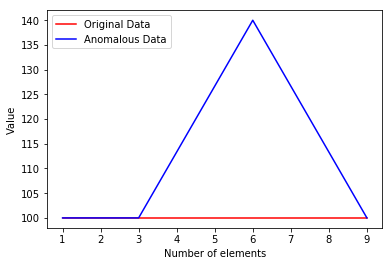
\includegraphics[totalheight=8cm]{anomaly-injection-identical-data.png}}
    \caption{Anomaly injection on an array containing all duplicate values. As an example this figure contains an array with all elements of the array having value '100'}
    \label{fig:ai_iden}
\end{figure}

We developed an anomaly injection tool to inject anomalies into our dataset to evaluate the accuracy of our anomaly detection methods. This tool manually injects anomalous data at any point of selection. We can even specify the number of anomalous points to inject, when we say injected anomalous points we mean, the existing data values are updated in such a way that the points represents values which looks unusual to the detection algorithms and the algorithms should be able to identify and classify them as anomalous. 

The developed tool has four parameters, \textbf{\textit{num}}, array containing the data, \textbf{\textit{x}}, is the parameter which lets the user to choose the percentage increase user wants to make to the data to look anomalous, \textbf{\textit{mid\_pos}}, the position in the data array where anomaly will be introduced, \textbf{\textit{count}}, will let the user control and keep count on the number of anomalies to put inside the data. One unique feature of this anomaly tool is, we do not need to introduce anomalies which looks obvious, instead, we have designed in such a way as to increase the value of selected point to  \textbf{\textit{x}}\% and additionally we provide the option to set the number of points to be made anomalous( \textbf{\textit{count}}). The count introduces those many anomaly points as the value itself on both sides of the selected point. 

The anomaly value is added to this range which follows a pattern of gradually increasing  from \textbf{\textit{mid\_pos}} - \textbf{\textit{count}} upto \textbf{\textit{mid\_pos}}  and then decreases gradually to   \textbf{\textit{mid\_pos}} + \textbf{\textit{count}} as shown in Fig \ref{fig:ai_iden} and  Fig \ref{fig:ai_rd}.  The distribution of original data and the anamolous data are plotted with simple line plot where x axis represents the index of the elements and y-axis represents the elements itself. The distribution in red depicts the behavior of unmodified elements and the distribution in blue depicts the behavior after injecting anamolies. Fig \ref{fig:ai_iden} shows the anomaly injection pattern for array containing all identical values and Fig \ref{fig:ai_rd} representing anomaly injection pattern for array containing random values. 

Two types of cases has been looked for in this area. One, all identical values elements and two, elements with random values. For identical values just for depicting the behavior of its distribution we used sample data and the results are shown in the Fig \ref{fig:ai_iden} and  Fig \ref{fig:ai_rd}. The point of insertion is at position 6 and number of anomaly points injected = 3 with the percentage of increase x=40\%, as you can see from Fig \ref{fig:ai_iden} the mid point at position 6 is increased 40\% (value = 140), either sides of it from position 3 to 6 and 6 to 9 are affected. Similarly to check with random data we used a list of random 10 numbers and injected 3 anomaly points on either sides from the selected middle point with x=40\%. We were successful in injecting the anomaly at the user provided point and range even for the random data as seen in the Fig \ref{fig:ai_rd}. 
\begin{figure}
\centerline{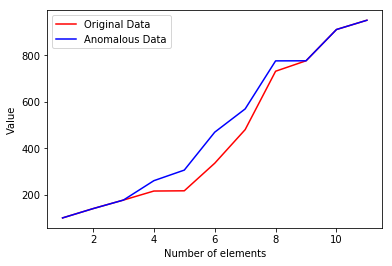
\includegraphics[totalheight=8cm]{anomaly-injection-random-data.png}}
    \caption{Anomaly injection on an array containing random data.}
    \label{fig:ai_rd}
\end{figure}

This anomaly injection tool can be used as a measure to check the accuracy of our methods. We know where we have injected the data and if the model is able to detect those anomalies which we have injected, then we can assure of a working anomaly detection method for our electrical data. With this tool in place we can also find out the number of false positives, false negatives, true positives as well as true negatives if any in our system. The design goal of this injection tool was mainly to evaluate the precision of our detection technique, to know how much deviation from the normal behavior can our model capture given the range of anomaly points. We assume our model to capture at least the mid point changes done while injecting the anomaly and nearby few points depending on the number of anomalies actually being injected.\\

At first, we take one week's Monday to Friday data and split it randomly into 80\% training data and remaining 20\% as the test data. We do not make any assumptions for supervised machine learning techniques here. The training and testing data are used with reference to unsupervised machine learning i.e the training set is composed of unmodified original datasets and the testing test is composed of modified datasets. The training set is used for modeling and learning our proposed algorithms, testing set is used to test the model(which are trained on the original dataset). Testing dataset will undergo anomaly injection procedure, to put few or may be more than few anomalous points. 

The anomaly injection tool is our own contribution to modify the datasets to contain abnormal values in a pre-defined fashion, the description of this tool is explained in Chapter 6. The percentage split is just random considering that the training dataset should be more than the testing dataset. We can choose anything between 50-50 split to 60-40, 70-30, or 80-20 depending on the size of the dataset. Since we have taken one week's data we want to capture most of the statistical values and hence decided to go with 80-20 split. We would also look into evaluating against 70-30 split in future or if the results are not as expected. For this we use the sklearn library's model\_selection.train\_test\_split() function which takes data and percentage variable ( which should be between 0 and 1) as parameters. The percentage variable if set to 0.5 gives us 50 percent training and 50 percent testing split of the data. Similarly, if the variable takes 0.6 then its a 60-40 split and so on. \\

\section{PCA residual space approach:}
PCA subspace projection is applied to data that have undergone random projection. Two key observations motivate this proposal. First, the computational complexity of PCA, when computed using the standard approach based on the singular value decomposition, scales like $O(l^3 + l^2n)$, where \textit{l} is the dimensionality of the data and \textit{n} is the sample size. Thus, use of the PCA subspace method is increasingly less feasible with the ever-increasing size and dimensions of modern data sets. Similar implementation has been already done in \cite{geijerlog}. 
\\
\section{GMM clustering approach:}

\label{sec:Impl}